
\part[Algoritmos sequenciais, condicionais e com repetições]
{Algoritmos sequenciais, condicionais e com repetições}


\chapter[Algoritmos sequenciais]
{Algoritmos sequenciais}



\section{Resumo}

Estrutura sequencial é um conjunto de instruções que serão executadas em sequência. A sequência de cada instrução deve ser seguida apara a realização de uma tarefa.
Neste capítulo, serão apresentados diversos exemplos mostrando como utilizar a playCB para plotar geometrias ou gráficos.


%\begin{chapreferences}{1.}
%\bibliography{playcb}
%\bibliographystyle{plain}
%\nocite{cbook}
%\nocite{sb6}
%\nocite{glfw}
%\nocite{cppbook}

%\end{chapreferences}

% \begin{chapreferences}{1}

% \bibitem{sb6}
% {\em OpenGL SuperBible}.
% \newblock Pearson Education Inc, 6 edition, 2014.

% \bibitem{glfw}
% Marcus Geelnard and Camilla Berglund.
% \newblock {\em GLFW - Reference guide}, 2010.
% \newblock API version 2.7.

% \bibitem{cbook}
% Brian~W. Kernighan and Dennis~M. Ritchie.
% \newblock {\em The C Programming Language}.
% \newblock 1989.

% \bibitem{cppbook}
% Stanley~B. Lippman, Josés Lajoile, and Barbara Moo.
% \newblock {\em C++ Primer}.
% \newblock 2013.
% \end{chapreferences}


\section{Plano Cartesiano}
\begin{figure}[ht]
  \centerline{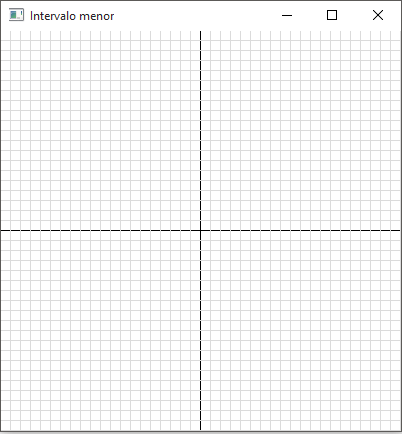
\includegraphics[width=.5\textwidth]{img/cap1_ex1.png}}
  \caption{Plano Cartesiano de -100 à 100}
  \label{fig:cap01_ex1}
\end{figure}
Esta prática se refere a exibir um Plano Cartesiano na tela com espaçamento de 5 em 5 unidades, tanto no eixo x quanto no eixo y. Com ela, o aluno poderá notar a importância da ordem de chamada de funções da playCB e a necessidade das funções \emph{AbreJanela} e \emph{Desenha}, além de verificar, com um exemplo simples, se a playCB foi corretamente bem instalada.
\lstinputlisting[caption=Código fonte de Plano Cartesiano, style=customc, label=lst:cap01_ex1]{src/ex1_PrimeiraJanela.cpp}

\section{Boneco Palito}
\begin{figure}[ht]
  \centerline{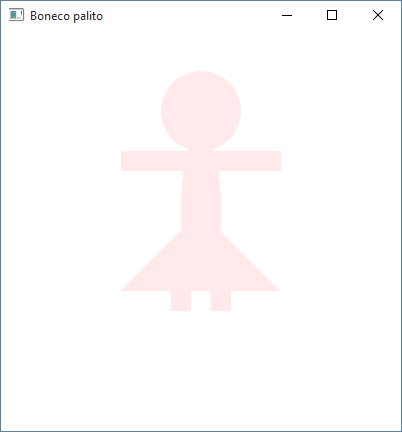
\includegraphics[width=.5\textwidth]{img/cap1_ex3.png}}
  \caption{Boneco Palito}
  \label{fig:cap01_ex1}
\end{figure}
Esta prática se refere a exibir um boneco palito e praticar todas as geometrias pré-definidas existentes na playCB. Os argumentos de cada função podem ser consultados no Guia de Referência da playCB \footnote{\url{http://pt-br.playcb.wikia.com/wiki/Categoria:Geometrias}}
\lstinputlisting[caption=Código fonte do boneco palito, style=customc, label=lst:cap01_ex1]{src/ex3_boneco.cpp}

\section{Estrela de Davi}
\begin{figure}[ht]
  \centerline{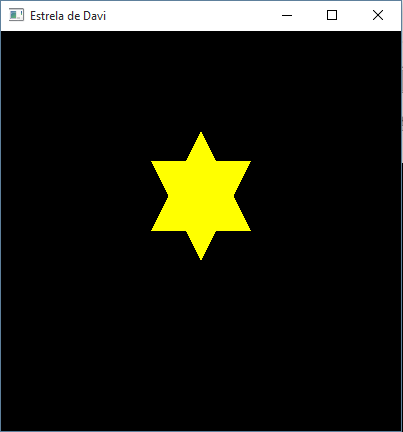
\includegraphics[width=.5\textwidth]{img/cap1_ex2.png}}
  \caption{Estrela de Davi}
  \label{fig:cap01_ex1}
\end{figure}
Esta prática se refere a exibir a estrela de Davi, feita com dois triângulos. Um triângulo foi criado com a função \emph{CriaTriangulo} e o outro com a função \emph{CriaPoligono}. Verificamos nesta prática os argumentos de \emph{CriaTriangulo} (base, altura e ponto esquerdo de referência) e, como não há como ter altura negativa, teve a necessidade de criar um polígono definido pelos três pontos \emph{p1, p2} e \emph{p3} para criar-se um triângulo \emph{de cabeça pra baixo}.
\lstinputlisting[caption=Código fonte da Estrela de Davi, style=customc, label=lst:cap01_ex1]{src/ex2_davi.cpp}

